%--------------PREAMBLE----------------------------------------------------------------------


\documentclass[12pt]{beamer}
\usetheme{boadilla}


\usepackage{ulem,bm,amsmath,bbm,amsfonts,nicefrac,latexsym,amsmath,amsfonts,amsbsy,amscd,amsxtra,amsgen,amsopn,bbm,amsthm,amssymb,graphicx} % you may include additional packages should you need them




\newcommand{\R}{\mathbb{R}}    % the real numbers


\title{Three Slide Introduction}
%\subtitle{PhD Title: Understanding the Information Content in Diverse Observations of Forest Carbon Stocks and Fluxes for Data %Assimilation and Ecological Modeling.\\ \newline{Supervised by Tristan Quaife.}}
\author{Ewan Pinnington}
\date{\vspace{-20mm}}

\begin{document}



%--------------TITLE SLIDE-----------------------------------------------------------------
\frame{

\maketitle
\vspace{-20mm}
\center{PhD student at Reading University in the UK}
\vspace{2mm}
\center{PhD Title:

 Understanding the Information Content in Diverse Observations of Forest Carbon Stocks and Fluxes for Data Assimilation and Ecological Modeling}


}


%--------------SLIDE 1-----------------------------------------------------------------
\section{DALEC 4DVAR}
\frame{\frametitle{4DVAR with DALEC}

\begin{figure}[h!]
    \centering
    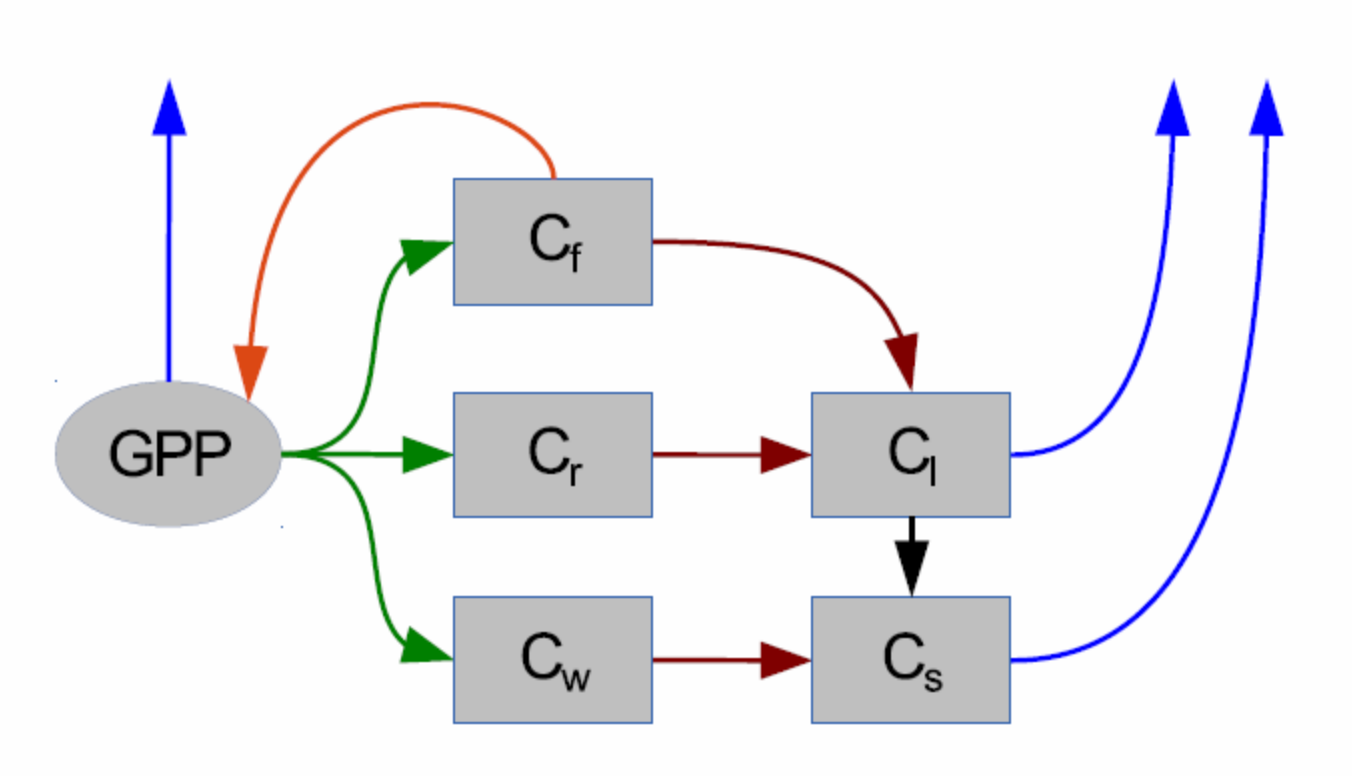
\includegraphics[width=0.5\textwidth]{DALECpic.png}
   % \caption{DALEC carbon balance model, (foliage ($C_f$), fine roots ($C_r$), woody biomass ($C_w$), litter ($C_l$) and soil organic matter ($C_s$)). The gross primary production function ($GPP$) uses meteorological driving data and the site's leaf area index (a function of $C_f$) to calculate the total amount of carbon to be allocated at a daily time step. }
    \label{fig:DALEC_mod}
\end{figure}

The DALEC model is coded up in a 4DVAR data assimilation scheme with cost function and gradient to be minimised where,

\[
J= \frac{1}{2} (\textbf{x}_0-\textbf{x}_B)^{T}\textbf{B}^{-1}(\textbf{x}_0-\textbf{x}_B)+\frac{1}{2}\sum\limits_{i=0}^n(\textbf{y}_i-\underline{h}_i(\textbf{x}_i))^{T}\textbf{R}_i^{-1}(\textbf{y}_i-\underline{h}_i(\textbf{x}_i))
\\ \bigtriangledown J  = \textbf{B}^{-1}(\textbf{x}_0-\textbf{x}_B)-\sum\limits_{i=0}^n\textbf{M}_{i,0}^{T}\textbf{H}_{i}^{T}\textbf{R}_i^{-1}(\textbf{y}_i-\underline{h}_i(\textbf{x}_i)).
\]
}

%--------------SLIDE 7-----------------------------------------------------------------
\frame{
\begin{figure}[h!]
    \centering
    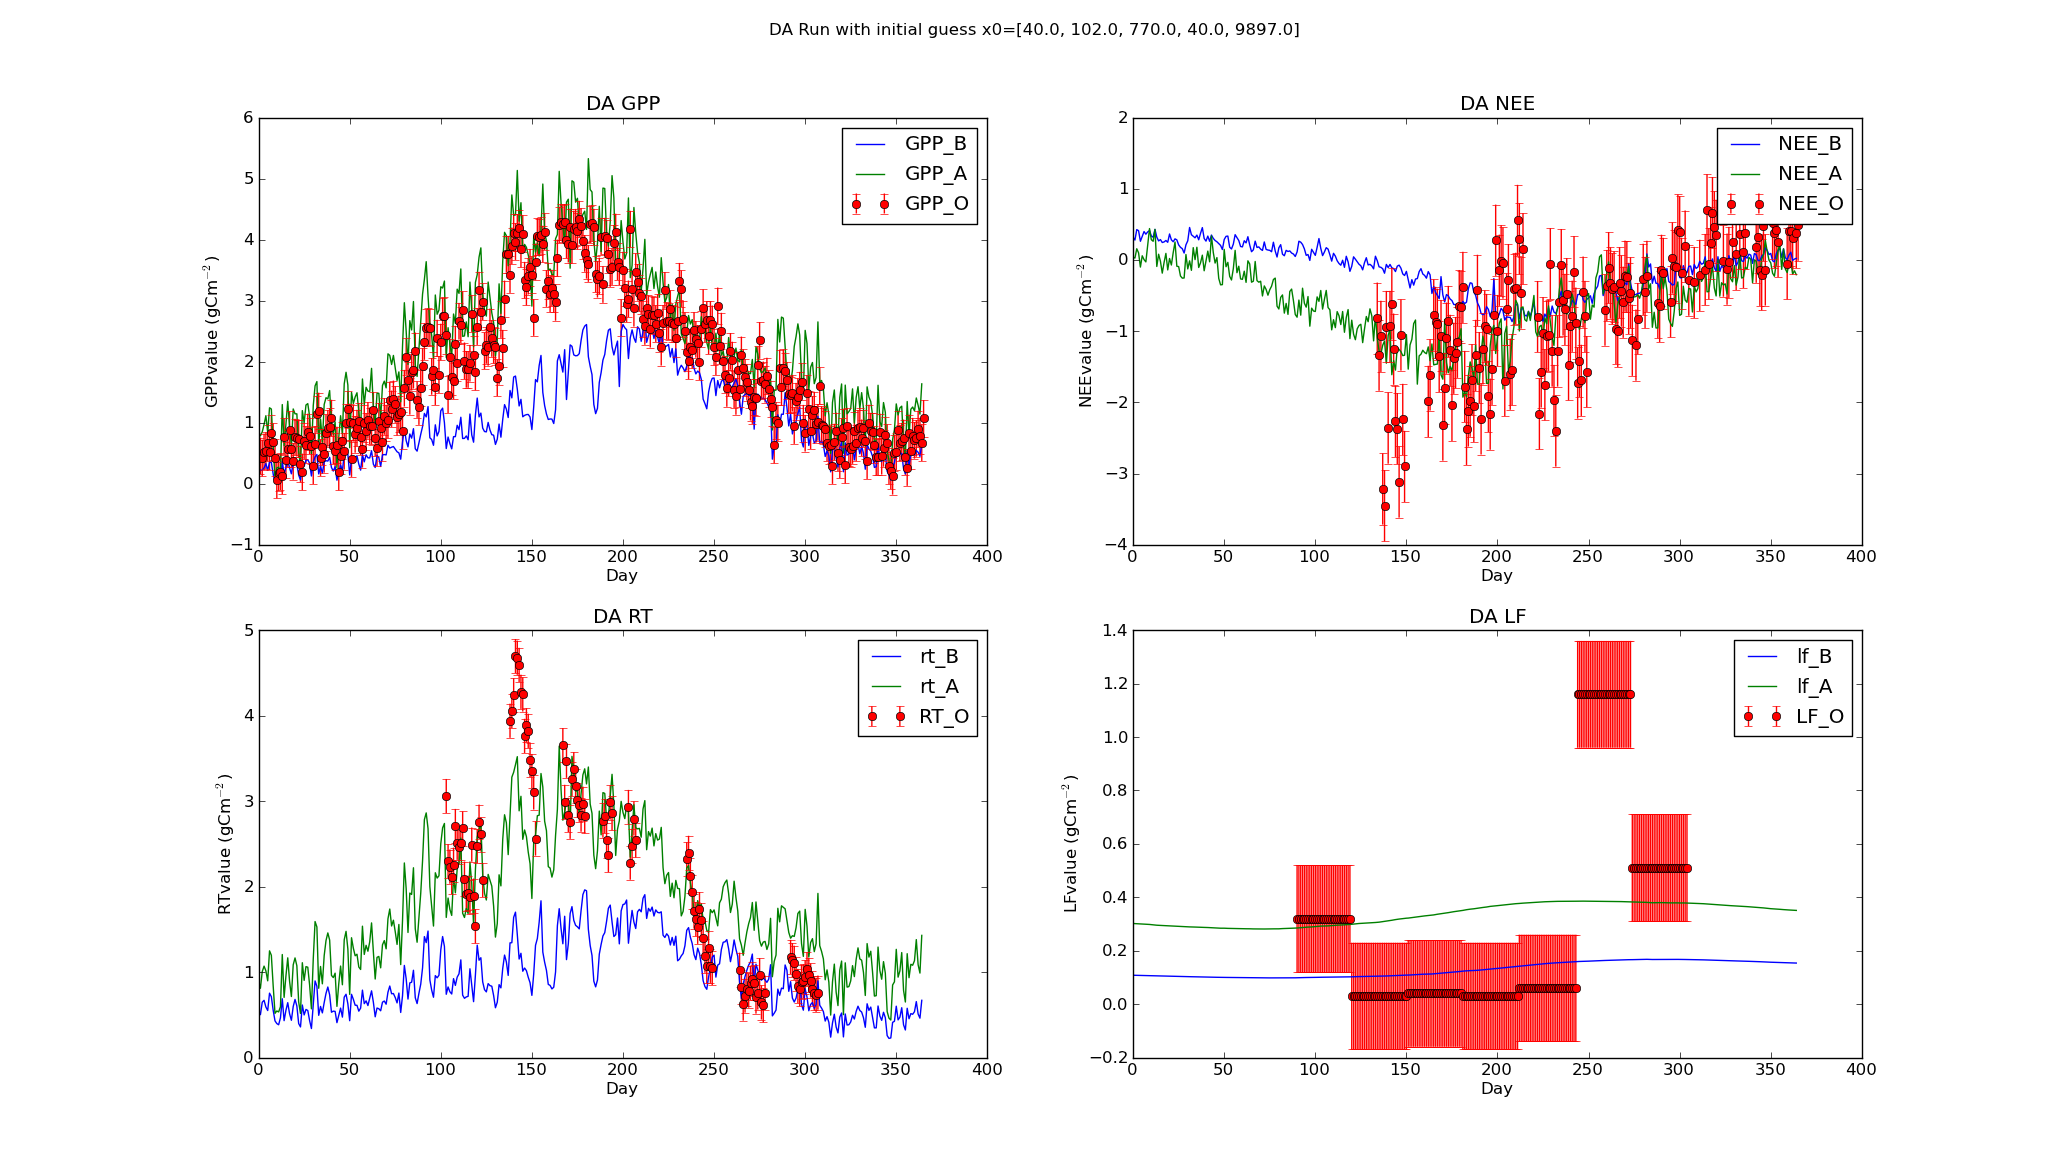
\includegraphics[width=1.04\textwidth]{DA_code_NEEonlybetterlabel.png}
    \caption{4DVAR DALEC with a 365 day assimilation window and only observations of NEE assimilated. }
    \label{fig:DALEC2_mod}
\end{figure}
}

\end{document}